\documentclass[11pt,a4paper]{report}

\usepackage[utf8]{inputenc}
\usepackage{graphicx}
\usepackage{float}
\usepackage{booktabs}
\usepackage{geometry}
\usepackage{setspace}
\usepackage{fancyhdr}
\usepackage{caption}
\usepackage{array}
\usepackage{longtable}
\usepackage{amsmath}
\usepackage{hyperref}

\geometry{
    a4paper,
    left=2.5cm,
    right=2.5cm,
    top=2.5cm,
    bottom=2.5cm
}

\setstretch{1.15}

\hypersetup{
    colorlinks=true,
    linkcolor=black,
    urlcolor=blue,
    citecolor=black
}

\pagestyle{fancy}
\fancyhf{}
\fancyhead[L]{Data Science Project Report}
\fancyhead[R]{Pharmaceutical Dispensing Analysis}
\fancyfoot[C]{\thepage}

\renewcommand{\headrulewidth}{0.4pt}

\begin{document}

% =========================================================
% TITLE PAGE
% =========================================================

\begin{titlepage}

\centering

\vspace*{2cm}

{\Huge \textbf{Exploratory Analysis of Pharmaceutical Dispensing Data in New Zealand}\par}

\vspace{1.5cm}

{\Large Data Science Project Report\par}

\vspace{2cm}

{\large
\textbf{Student Name:} A,B,C,D
\par}

\vspace{0.5cm}

{\large
\textbf{Student ID:} XXXXXXXX
\par}

\vspace{1cm}

{\large
\textbf{Course:} DATA301
\par}

\vspace{0.5cm}

{\large
\textbf{Group Project}
\par}

\vfill

{\large
Victoria University of Wellington
\par}

\vspace{0.5cm}

{\large
2026
\par}

\end{titlepage}


% =========================================================
% CONTENTS
% =========================================================

\tableofcontents

\clearpage


% =========================================================
% CHAPTER 1
% =========================================================

\chapter{Background and Data}

\section{Background}

This project analyses pharmaceutical dispensing data from New Zealand between 2021 and 2024. The dataset records initial pharmaceutical dispensings across different therapeutic groups and health districts.

The analysis focuses on Therapeutic Group Level 2 categories and examines how dispensing patterns differ between therapeutic groups, years, and health districts.

Pharmaceutical dispensing data can provide useful information about patterns of medicine use across New Zealand. Looking at dispensing levels over time can help identify therapeutic groups with increasing or decreasing use, while comparing districts can show differences in dispensing activity across different parts of the country.

The main purpose of this exploratory data analysis is to identify important patterns in the dataset before carrying out any further statistical analysis.

\section{Data Description}

The main dataset contains information about pharmaceutical dispensing activity. The key variables used in this analysis include:

\begin{itemize}
    \item \textbf{TherapeuticGrp2}: Therapeutic Group Level 2 category.
    \item \textbf{District}: Health district where the dispensing was recorded.
    \item \textbf{YearDisp}: Year of dispensing.
    \item \textbf{NumDisps}: Number of initial dispensings.
    \item \textbf{NumPpl}: Number of people associated with the dispensing records.
    \item \textbf{NHIComp}: NHI completeness measure.
\end{itemize}

The analysis covers the years 2021 to 2024.

For the district-level analysis, the ``New Zealand'' total was removed. This was necessary because the national total is not an individual health district and including it would make comparisons between districts misleading.

\section{Data Preparation}

The variable \texttt{NumDisps} contains the number of initial dispensings. Some observations may be reported as ``<6''. These values do not provide an exact number and were therefore treated as missing when calculating numerical totals.

The dispensing variable was converted into a numeric variable called \texttt{NumDisps\_num}.

The district analysis included the 20 individual health districts and excluded the New Zealand total.

The data were then grouped by therapeutic group, year, and district to calculate total initial dispensings.

\section{Exploratory Analysis Approach}

Four main visualisations were used in this exploratory analysis.

First, the ten therapeutic groups with the highest total dispensing levels were identified.

Second, the changes in dispensing levels for these top ten groups were examined between 2021 and 2024.

Third, total dispensing levels were compared between health districts.

Finally, a heatmap was used to examine the relationship between the top ten therapeutic groups and the different health districts.


% =========================================================
% CHAPTER 2
% =========================================================

\chapter{Exploratory Data Analysis}

This chapter presents the main findings from the exploratory analysis of pharmaceutical dispensing data. The analysis focuses on the most frequently dispensed therapeutic groups, changes over time, differences between districts, and dispensing patterns across therapeutic groups and districts.


% =========================================================
% 2.1
% =========================================================

\section{Top 10 Therapeutic Groups}

Figure~\ref{fig:top10} shows the ten Therapeutic Group Level 2 categories with the highest total number of initial dispensings between 2021 and 2024.

\begin{figure}[H]
    \centering
    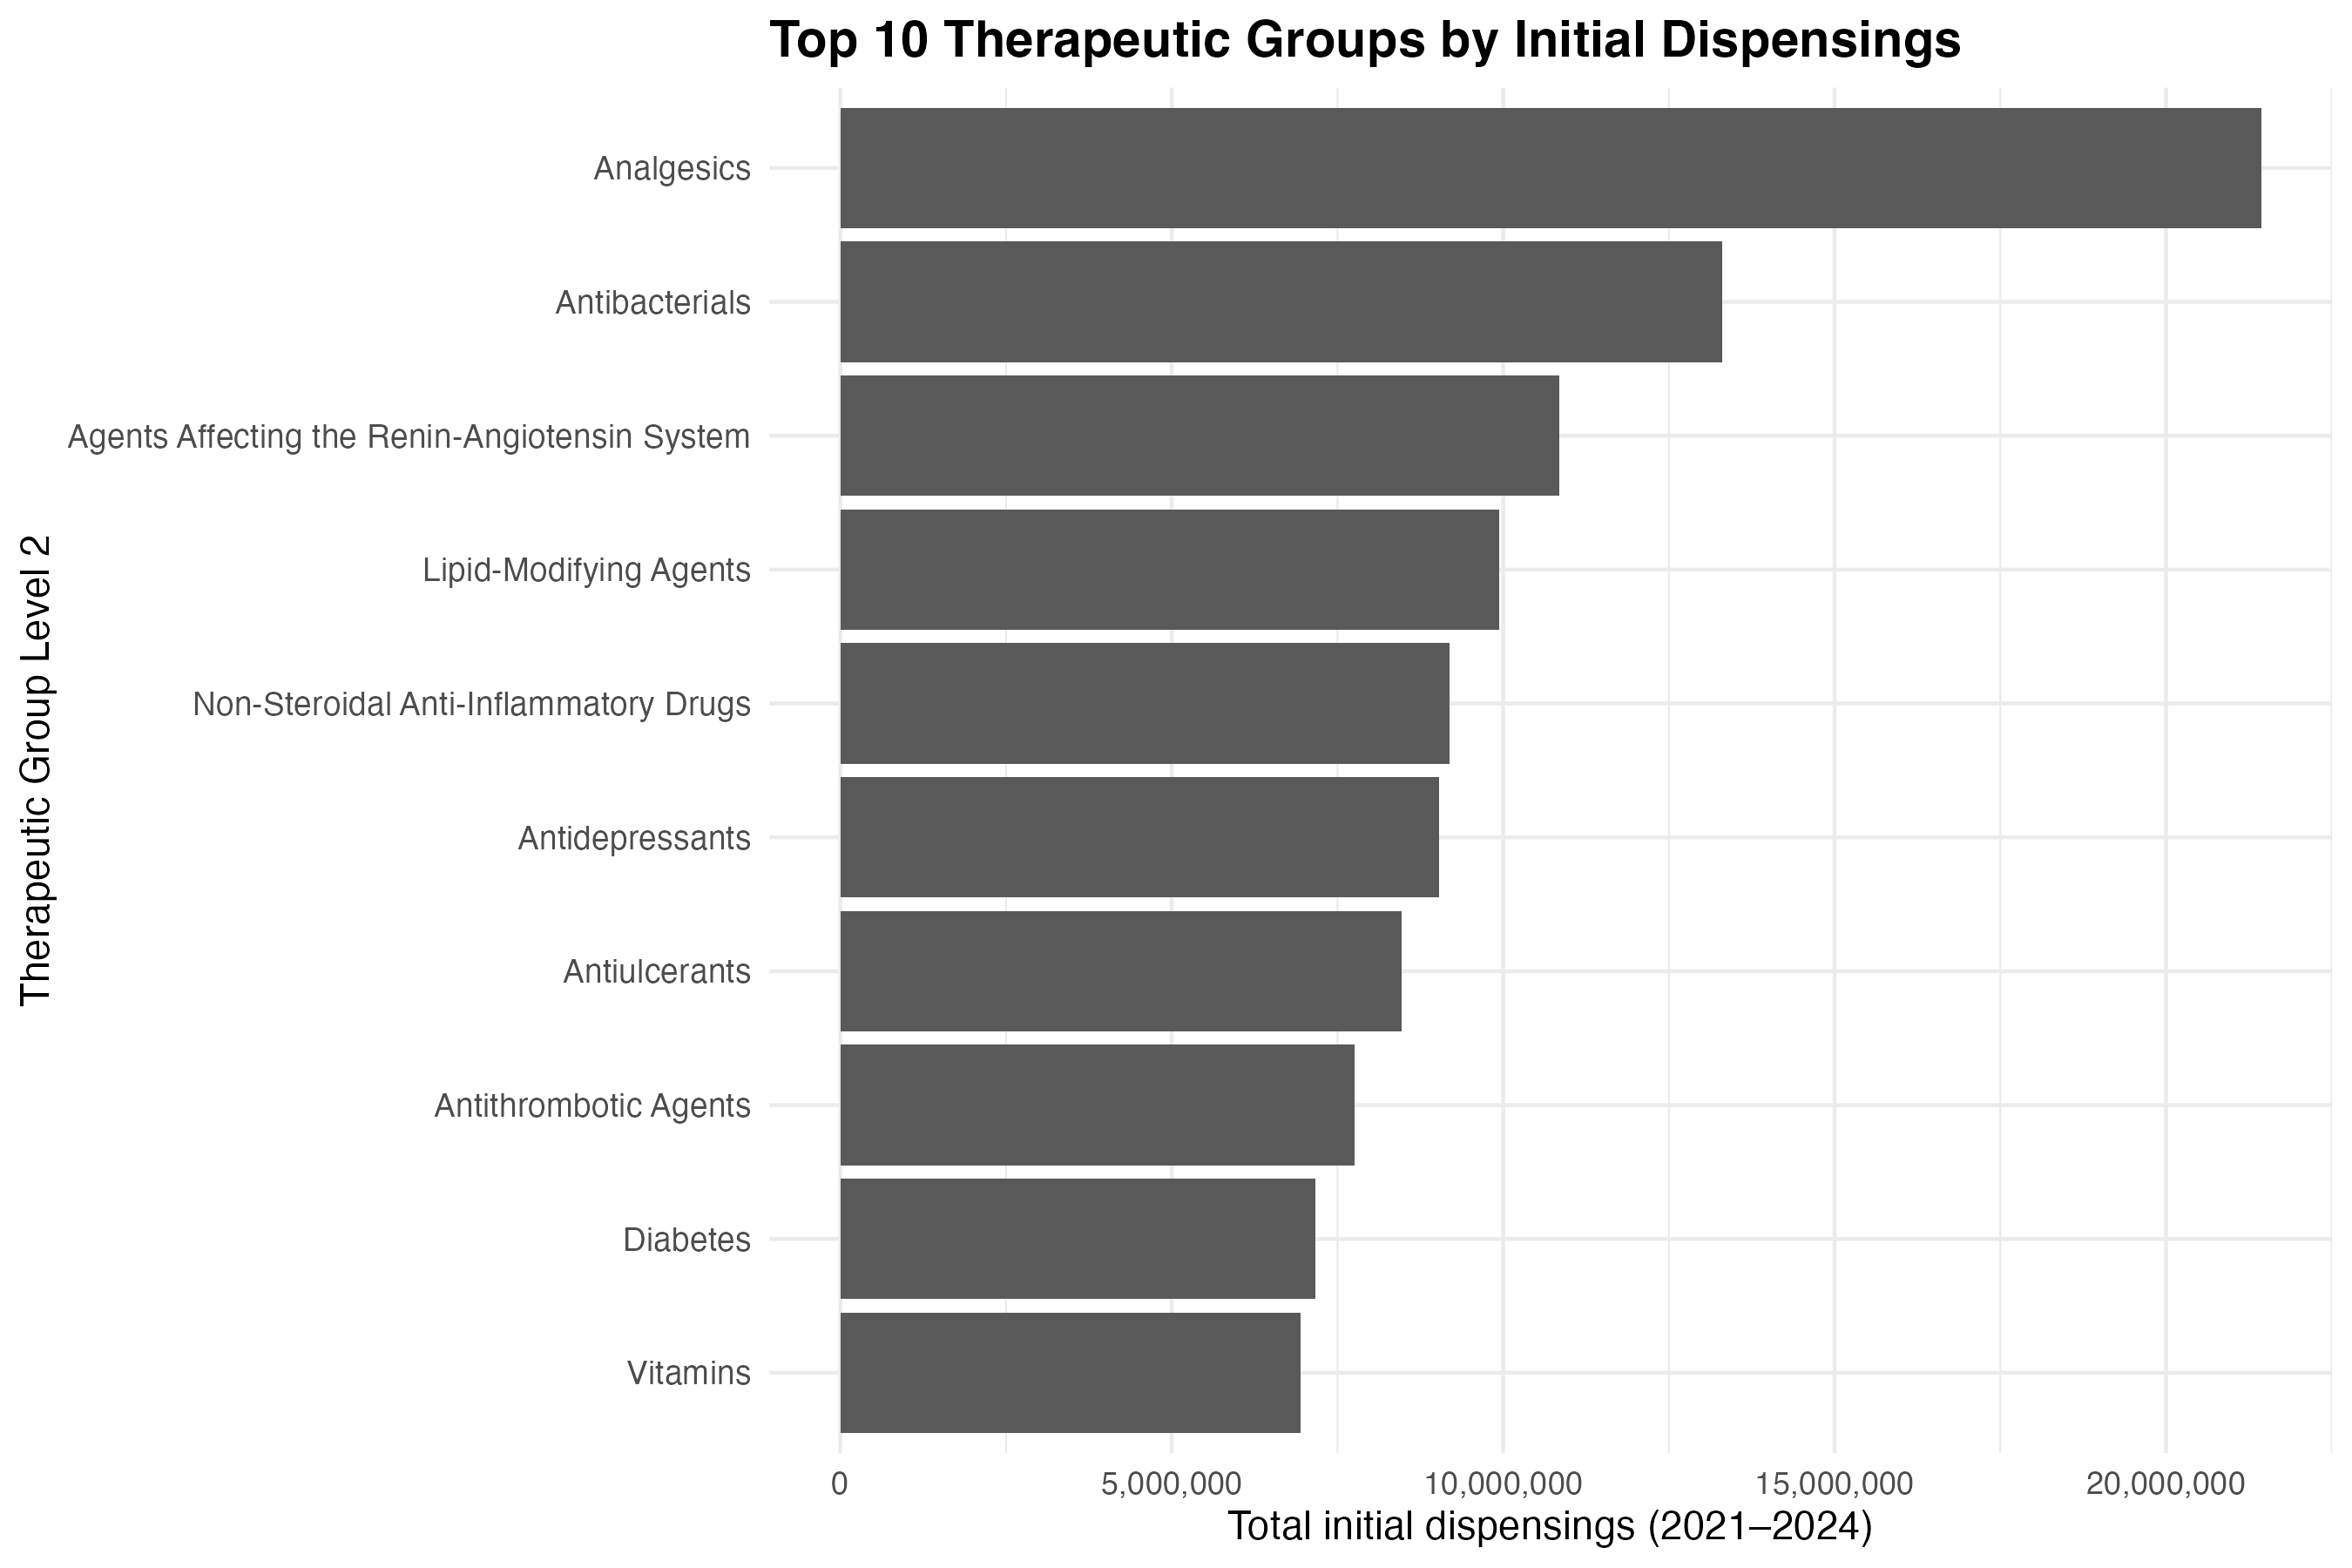
\includegraphics[width=0.90\textwidth]{top10_groups.png}
    \caption{Top 10 Therapeutic Groups by Initial Dispensings.}
    \label{fig:top10}
\end{figure}

Analgesics had the highest total number of initial dispensings, with approximately 21.4 million dispensings between 2021 and 2024.

Antibacterials were the second highest group, with approximately 13.3 million dispensings. Agents Affecting the Renin-Angiotensin System had approximately 10.9 million dispensings, while Lipid-Modifying Agents had approximately 9.9 million.

The ten highest dispensing groups were:

\begin{enumerate}
    \item Analgesics
    \item Antibacterials
    \item Agents Affecting the Renin-Angiotensin System
    \item Lipid-Modifying Agents
    \item Non-Steroidal Anti-Inflammatory Drugs
    \item Antidepressants
    \item Antiulcerants
    \item Antithrombotic Agents
    \item Diabetes
    \item Vitamins
\end{enumerate}

The results show that Analgesics were clearly the most frequently dispensed therapeutic group in the dataset.

\clearpage


% =========================================================
% 2.2
% =========================================================

\section{Changes in Dispensing Over Time}

Figure~\ref{fig:trend} shows the trends in initial dispensings for the top ten therapeutic groups from 2021 to 2024.

\begin{figure}[H]
    \centering
    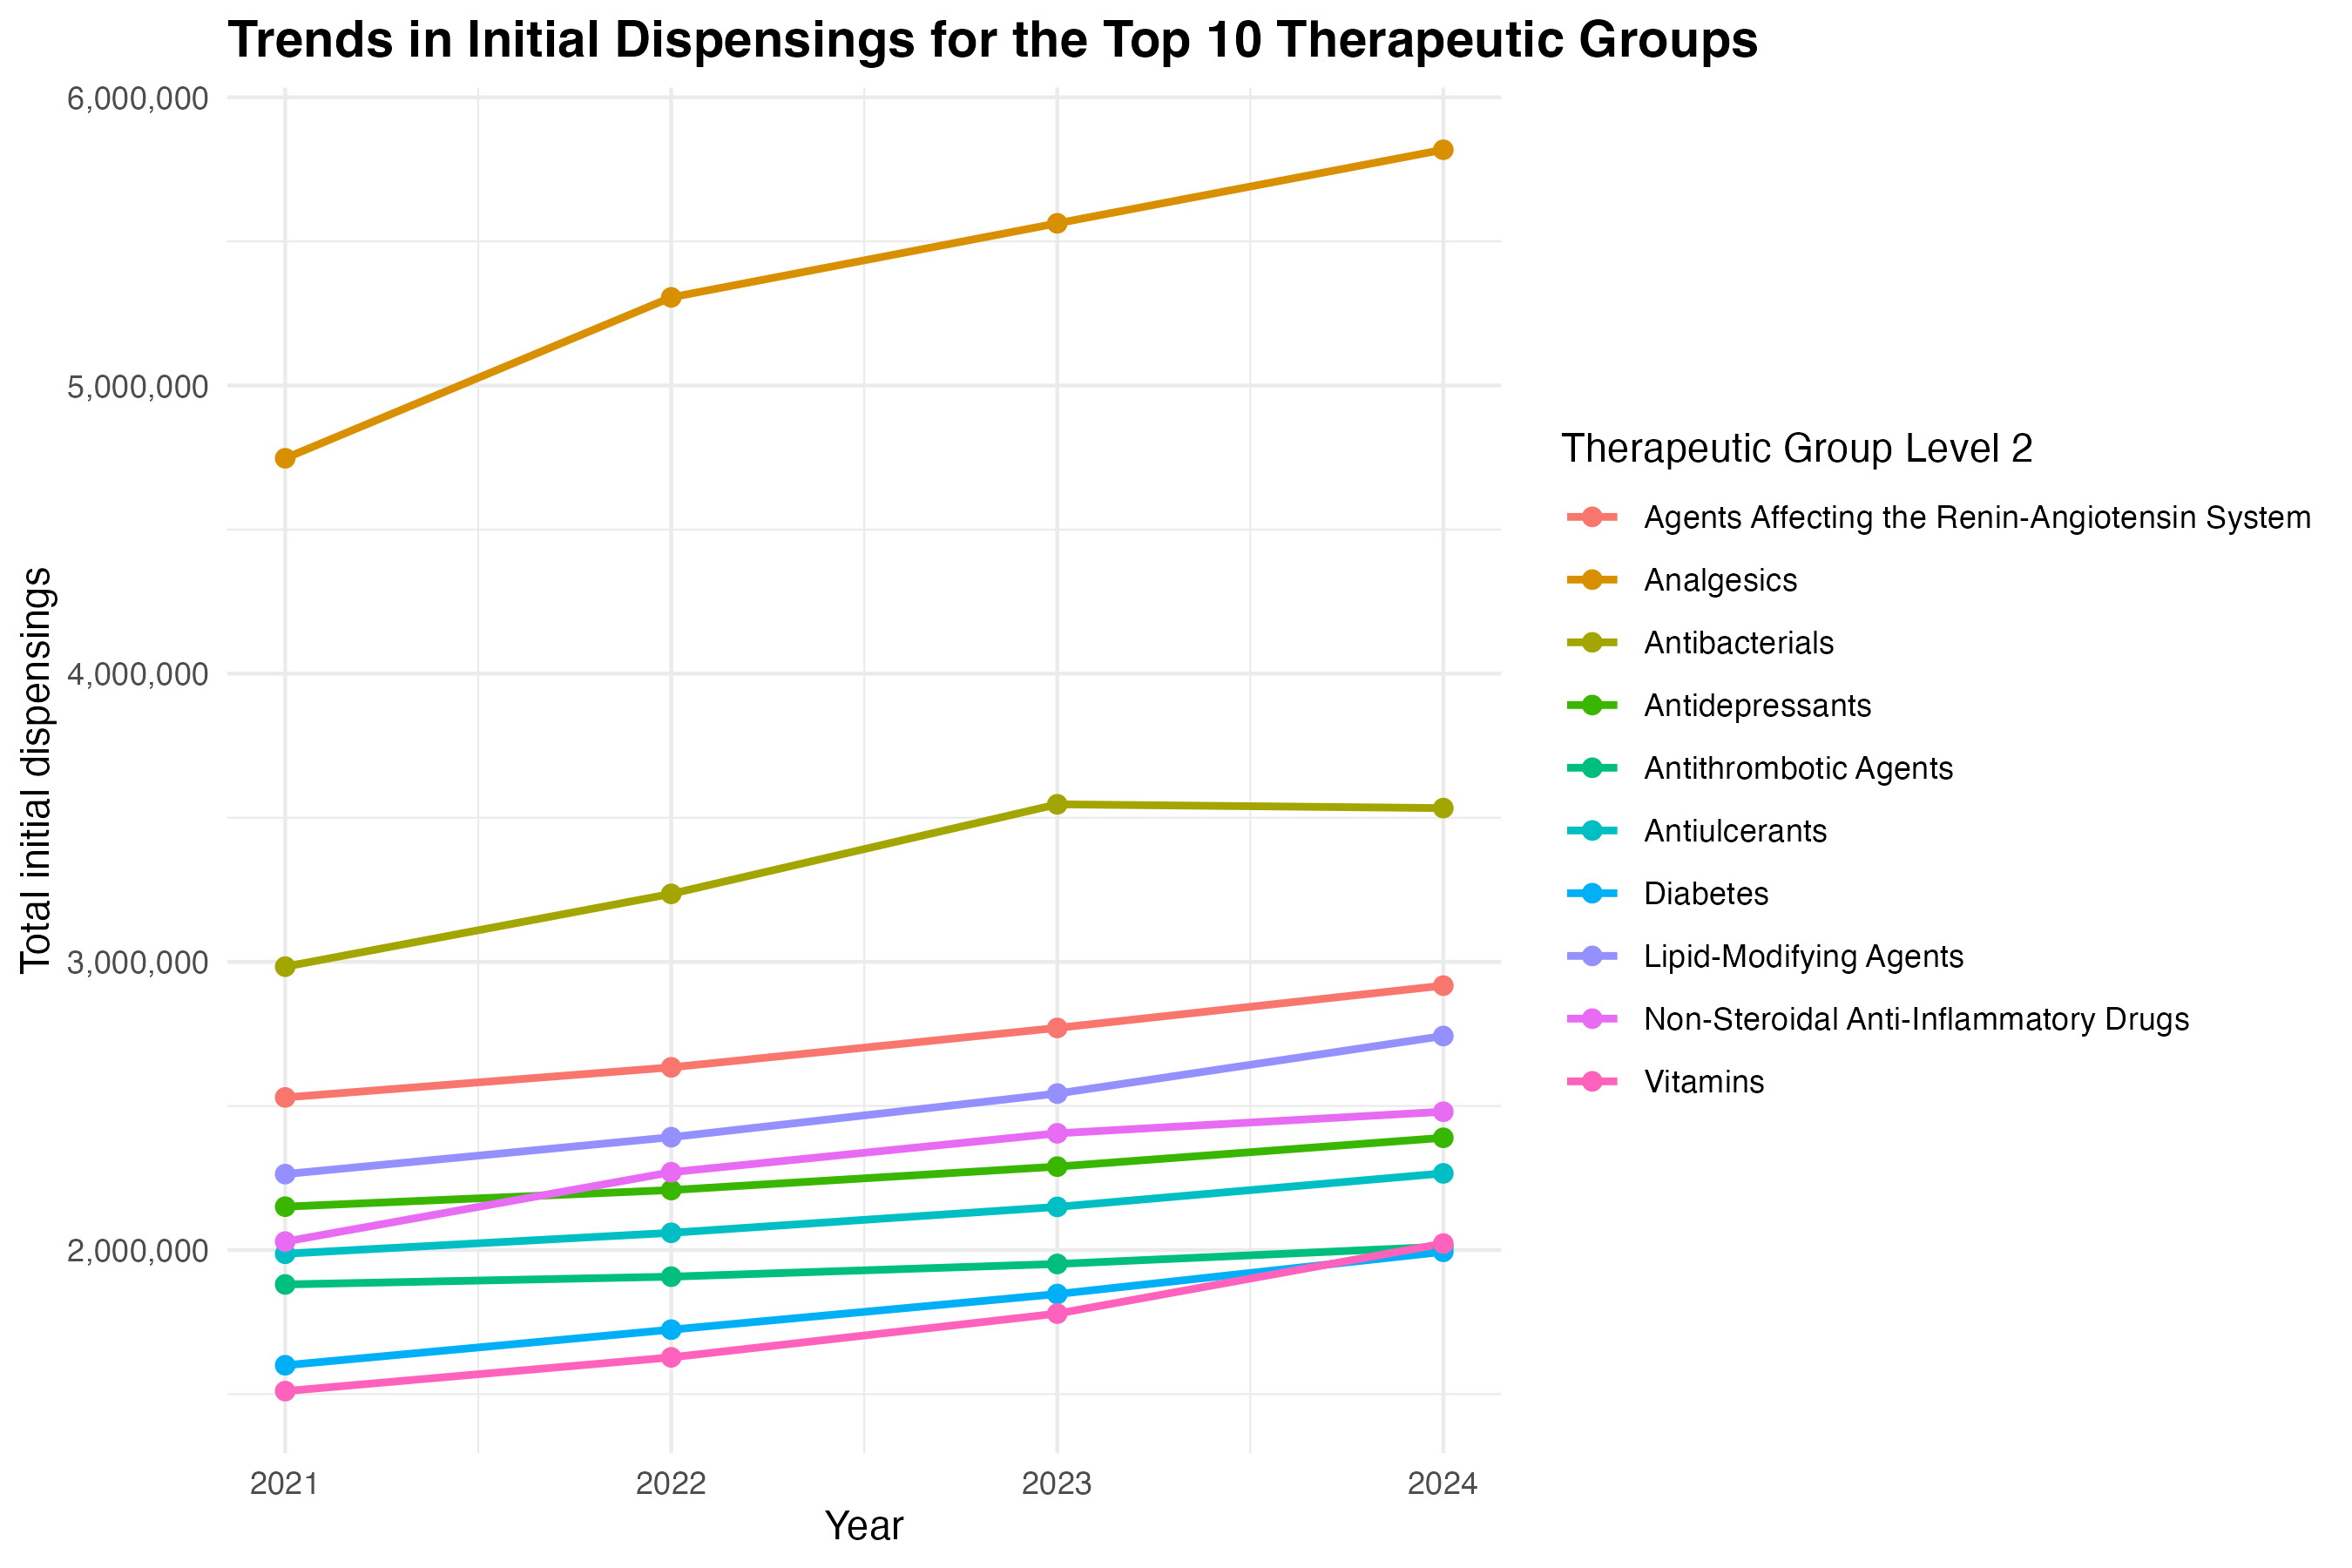
\includegraphics[width=0.95\textwidth]{trend_top10.png}
    \caption{Trends in Initial Dispensings for the Top 10 Therapeutic Groups.}
    \label{fig:trend}
\end{figure}

Overall, the dispensing levels of all ten top therapeutic groups increased between 2021 and 2024.

Analgesics showed the largest absolute increase. Dispensing increased from approximately 4.75 million in 2021 to approximately 5.82 million in 2024. This represents an increase of approximately 22.5\%.

Vitamins showed the largest percentage increase, rising by approximately 33.9\% between 2021 and 2024.

Diabetes also showed a relatively large increase of approximately 24.6\%. Lipid-Modifying Agents increased by approximately 21.2\%, while Non-Steroidal Anti-Inflammatory Drugs increased by approximately 22.2\%.

Antithrombotic Agents showed the smallest percentage increase, at approximately 7.0\%.

The overall pattern suggests that dispensing increased across all of the major therapeutic groups during the period studied.

\clearpage


% =========================================================
% 2.3
% =========================================================

\section{Differences Between Health Districts}

Figure~\ref{fig:district} compares total initial dispensings across the 20 individual health districts.

\begin{figure}[H]
    \centering
    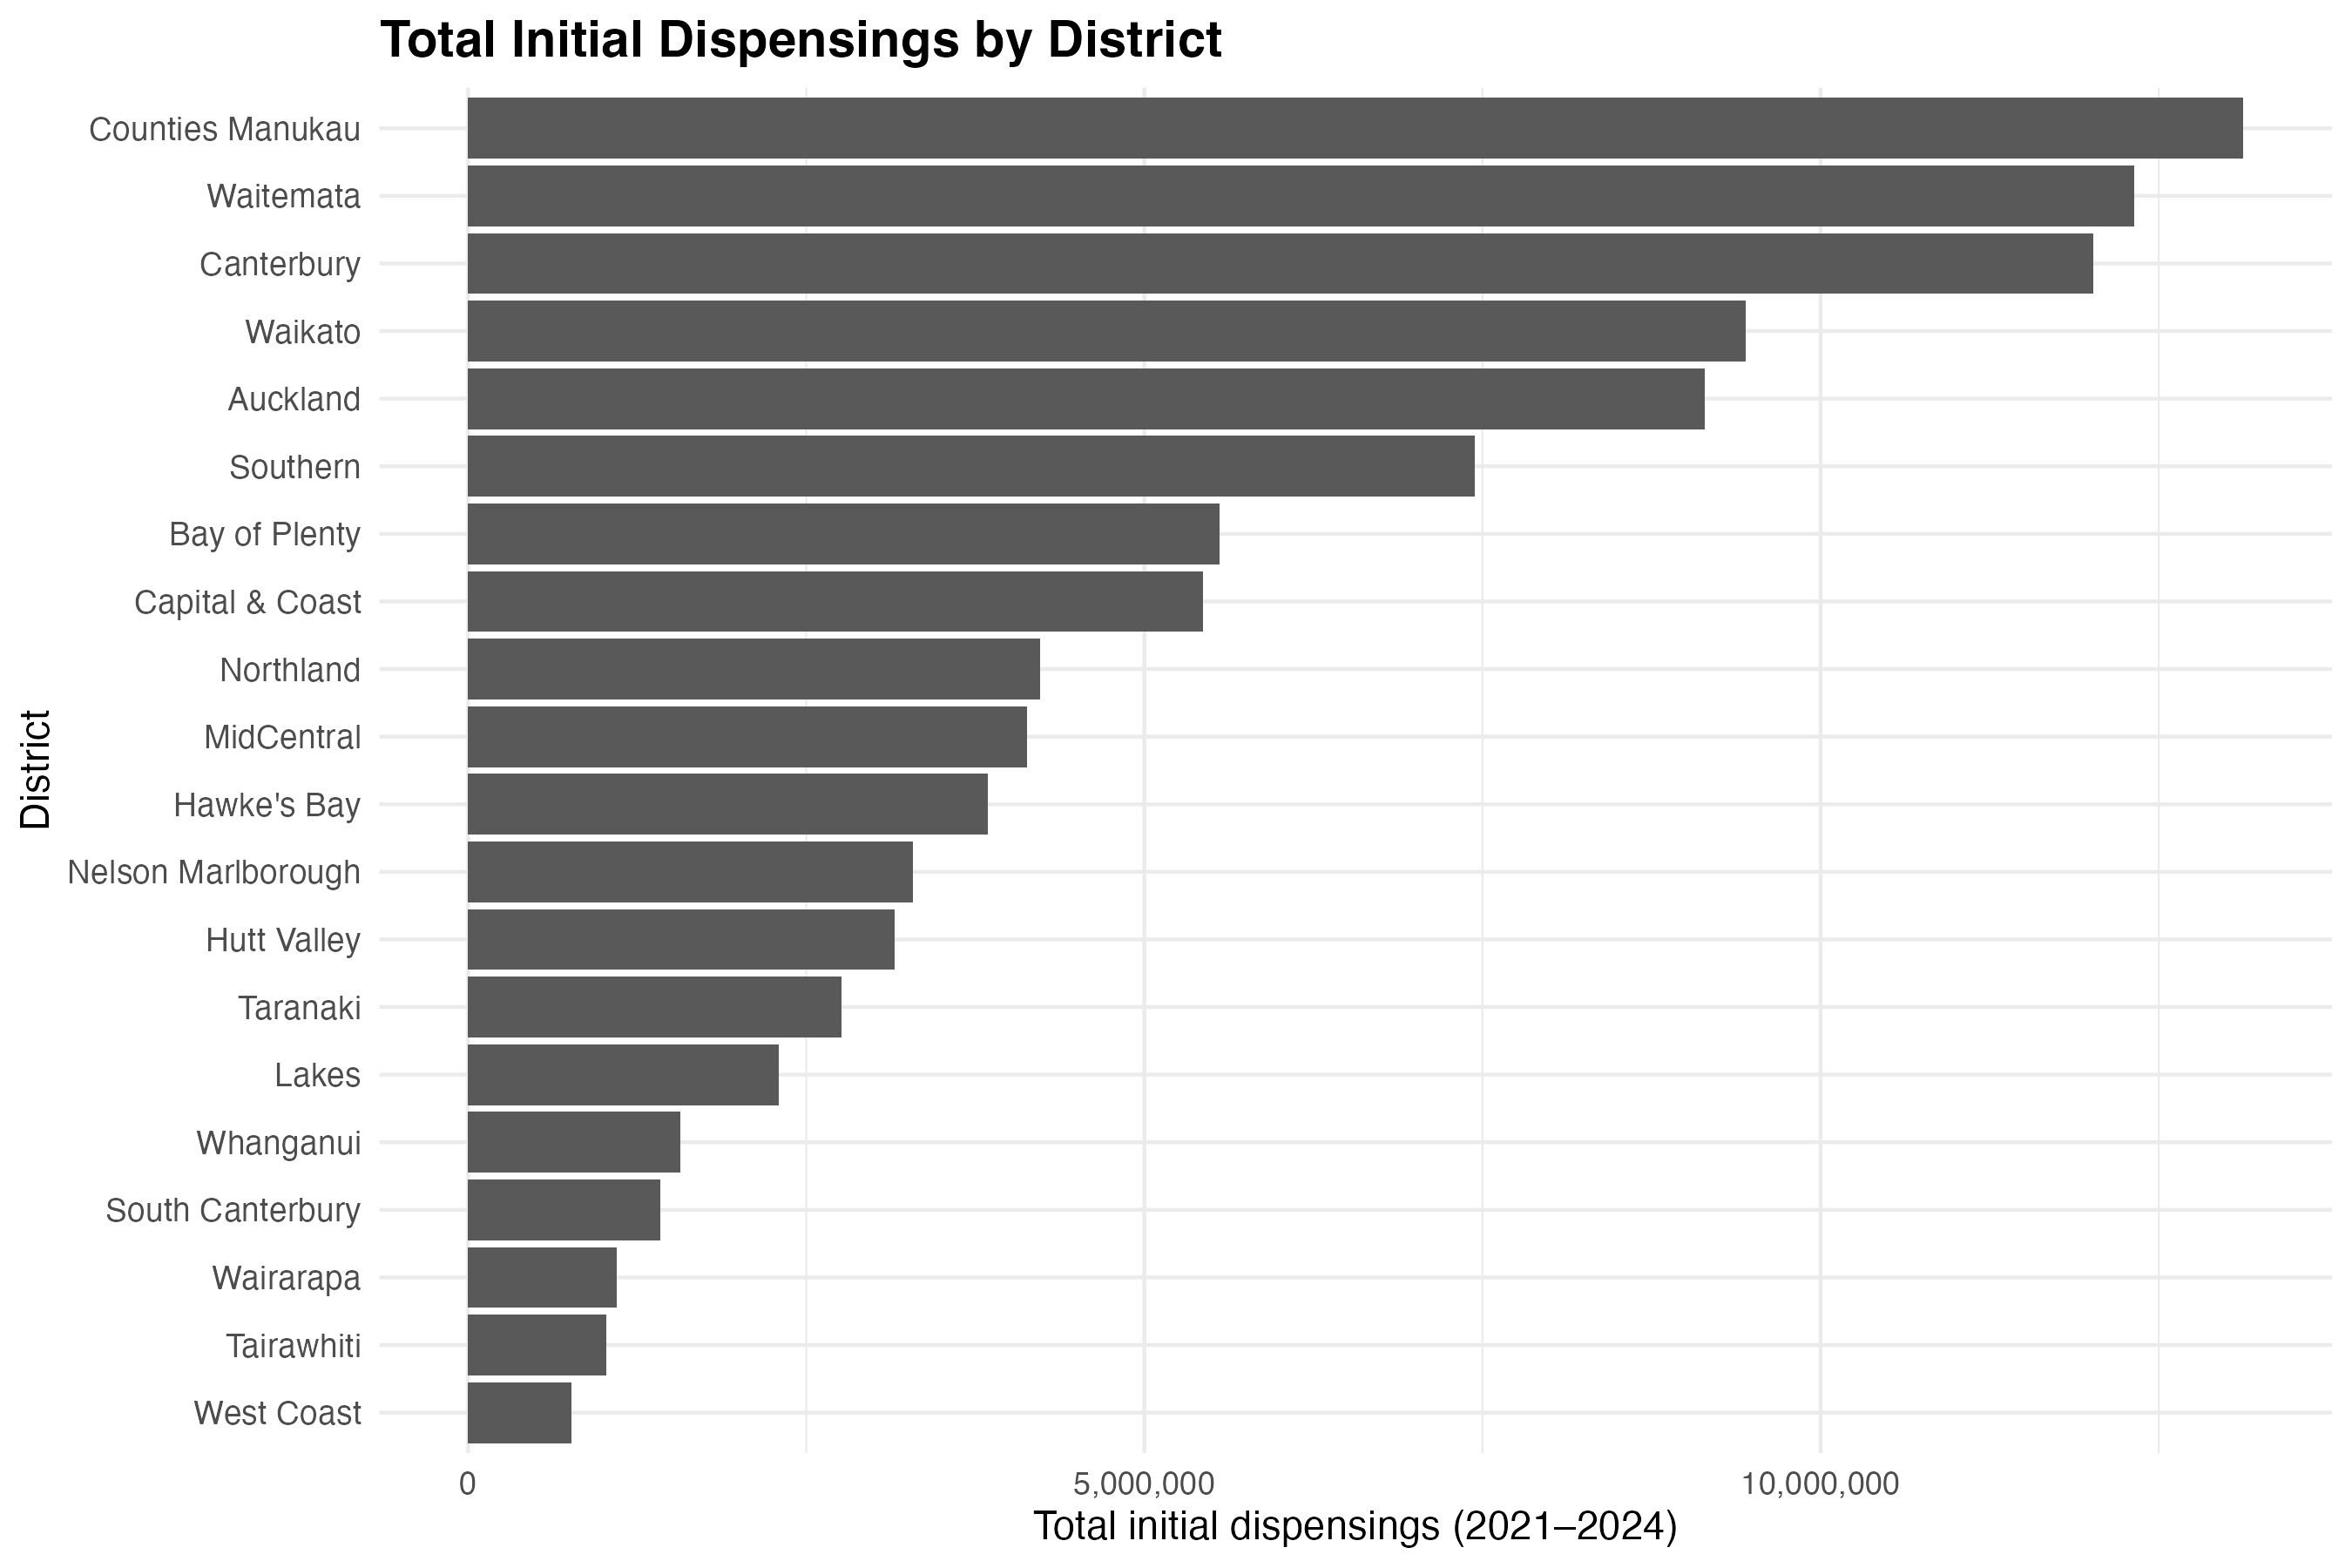
\includegraphics[width=0.90\textwidth]{district_total.png}
    \caption{Total Initial Dispensings by District.}
    \label{fig:district}
\end{figure}

The results show substantial differences between health districts.

Counties Manukau had the highest total dispensing level, with approximately 13.1 million initial dispensings between 2021 and 2024.

Waitemata was second with approximately 12.3 million, followed by Canterbury with approximately 12.0 million.

Waikato and Auckland were also among the districts with relatively high dispensing totals.

In contrast, West Coast had the lowest total, with approximately 0.77 million initial dispensings. Tairawhiti and Wairarapa also had relatively low totals.

The five districts with the highest total dispensing levels were:

\begin{table}[H]
\centering
\caption{Five Districts with the Highest Total Initial Dispensings}
\label{tab:highest}
\begin{tabular}{lr}
\toprule
\textbf{District} & \textbf{Total Dispensings} \\
\midrule
Counties Manukau & 13,125,771 \\
Waitemata & 12,320,411 \\
Canterbury & 12,019,022 \\
Waikato & 9,443,627 \\
Auckland & 9,143,739 \\
\bottomrule
\end{tabular}
\end{table}

The five districts with the lowest totals were:

\begin{table}[H]
\centering
\caption{Five Districts with the Lowest Total Initial Dispensings}
\label{tab:lowest}
\begin{tabular}{lr}
\toprule
\textbf{District} & \textbf{Total Dispensings} \\
\midrule
West Coast & 765,415 \\
Tairawhiti & 1,020,032 \\
Wairarapa & 1,101,108 \\
South Canterbury & 1,422,087 \\
Whanganui & 1,571,126 \\
\bottomrule
\end{tabular}
\end{table}

These differences should not automatically be interpreted as differences in medicine use by individuals. Larger districts may have larger populations, so population size is likely to contribute to the differences in total dispensing levels.

\clearpage


% =========================================================
% 2.4
% =========================================================

\section{Therapeutic Groups Across Districts}

Figure~\ref{fig:heatmap} presents a heatmap showing dispensing patterns for the top ten therapeutic groups across the 20 health districts.

\begin{figure}[H]
    \centering
    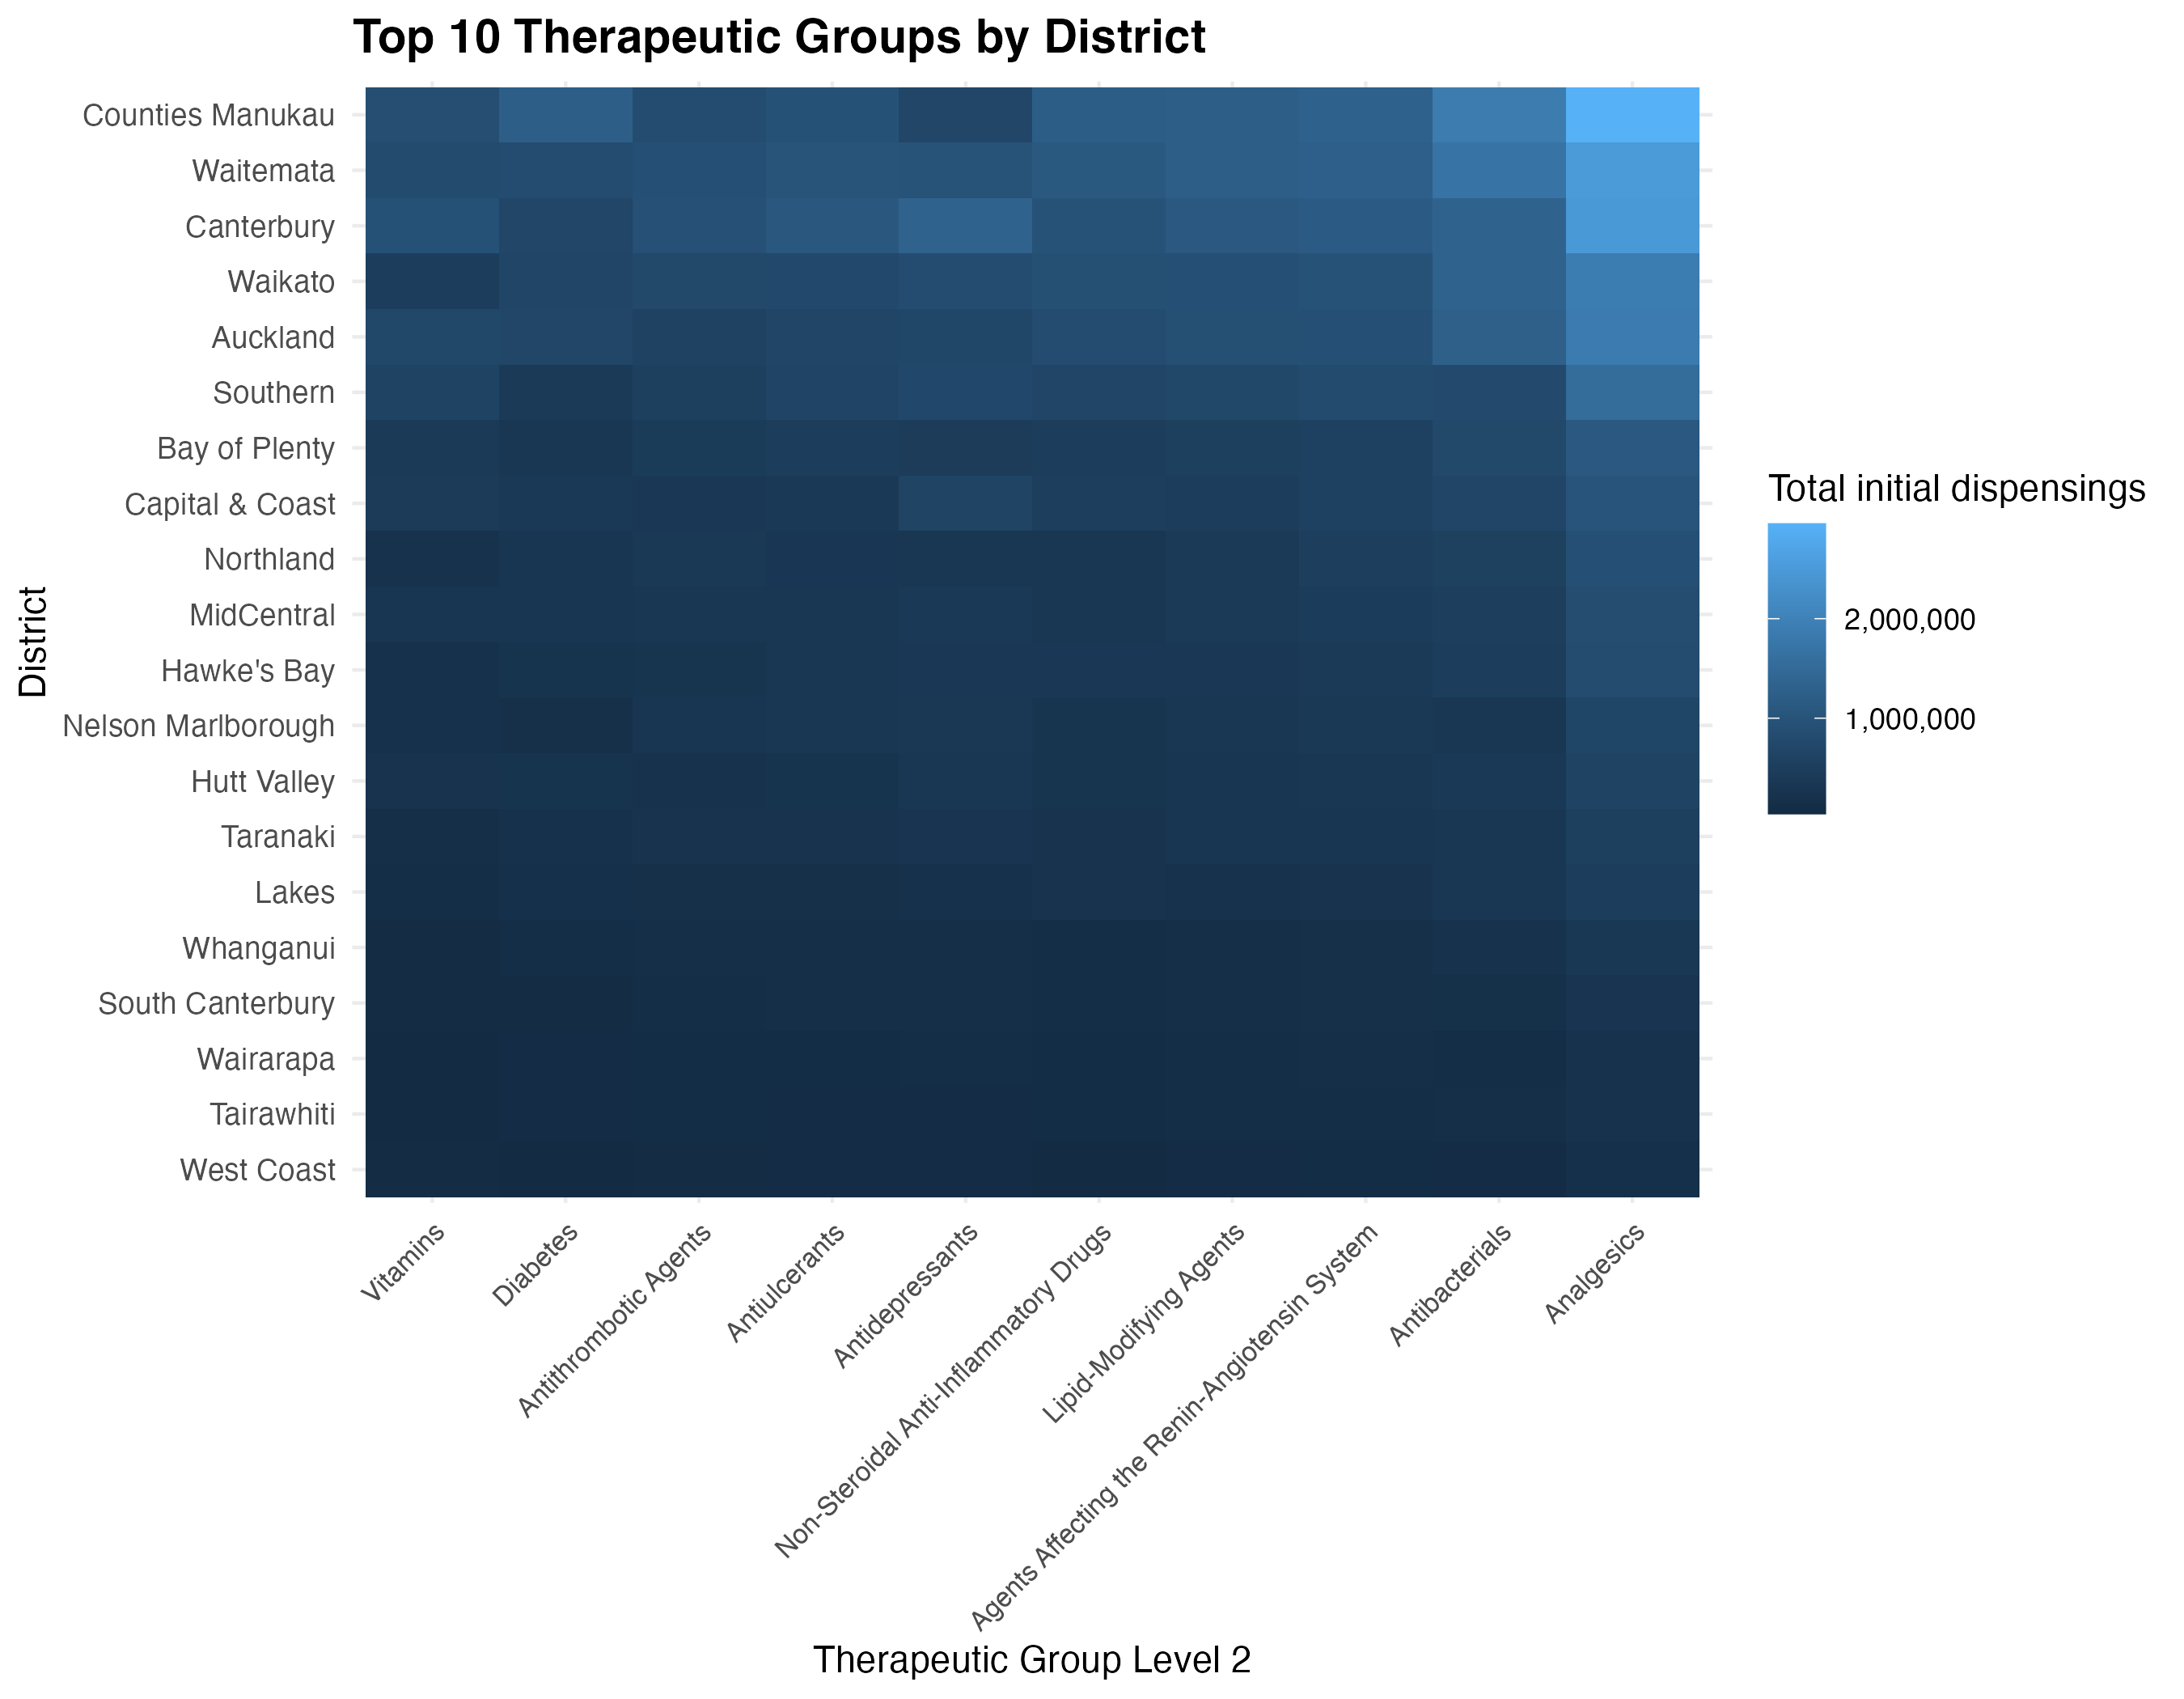
\includegraphics[width=0.95\textwidth]{district_top10.png}
    \caption{Top 10 Therapeutic Groups by District.}
    \label{fig:heatmap}
\end{figure}

The heatmap shows that dispensing levels vary across both therapeutic groups and districts.

Analgesics generally had high dispensing levels across many districts. Counties Manukau had the highest dispensing level for Analgesics, followed by Waitemata and Canterbury.

Antibacterials were also relatively high in several districts, particularly Counties Manukau and Waitemata.

The heatmap also shows that districts with lower overall dispensing totals generally had lower values across most of the top therapeutic groups.

This suggests that the overall district differences are not caused by a single therapeutic group. Instead, the differences appear across several major therapeutic categories.

The highest district and therapeutic group combinations were:

\begin{table}[H]
\centering
\caption{Highest District and Therapeutic Group Combinations}
\label{tab:combinations}
\begin{tabular}{llr}
\toprule
\textbf{District} & \textbf{Therapeutic Group} & \textbf{Dispensings} \\
\midrule
Counties Manukau & Analgesics & 2,954,966 \\
Waitemata & Analgesics & 2,507,433 \\
Canterbury & Analgesics & 2,479,564 \\
Waikato & Analgesics & 1,890,600 \\
Counties Manukau & Antibacterials & 1,868,958 \\
Auckland & Analgesics & 1,858,920 \\
Waitemata & Antibacterials & 1,681,852 \\
Southern & Analgesics & 1,533,063 \\
Canterbury & Antibacterials & 1,342,083 \\
Canterbury & Antidepressants & 1,324,674 \\
\bottomrule
\end{tabular}
\end{table}

The lowest combinations were mainly found in West Coast, Tairawhiti, and Wairarapa.

For example, Tairawhiti had only 37,835 dispensing records for Vitamins, while West Coast had 43,224 for Diabetes.

These results demonstrate that there are clear differences in dispensing patterns between districts.


% =========================================================
% CHAPTER 3
% =========================================================

\chapter{Key Findings and Discussion}

\section{Main Findings}

The exploratory analysis identified several important patterns in New Zealand pharmaceutical dispensing data.

First, Analgesics were the most frequently dispensed Therapeutic Group Level 2 category between 2021 and 2024, with approximately 21.4 million initial dispensings.

Second, all of the top ten therapeutic groups increased between 2021 and 2024. Analgesics had the largest absolute increase, while Vitamins had the largest percentage increase.

Third, dispensing levels varied substantially between health districts. Counties Manukau had the highest total dispensing level, while West Coast had the lowest.

Finally, the heatmap showed that differences between districts occurred across several therapeutic groups rather than being limited to one category.

\section{Changes Between 2021 and 2024}

The change analysis provides a useful comparison of dispensing levels over time.

\begin{table}[H]
\centering
\caption{Changes in the Top 10 Therapeutic Groups Between 2021 and 2024}
\label{tab:change}
\begin{tabular}{lrrr}
\toprule
\textbf{Therapeutic Group} &
\textbf{2021} &
\textbf{2024} &
\textbf{Change (\%)} \\
\midrule
Analgesics & 4,747,437 & 5,817,975 & 22.5 \\
Antibacterials & 2,983,307 & 3,533,539 & 18.4 \\
Vitamins & 1,510,462 & 2,022,481 & 33.9 \\
Lipid-Modifying Agents & 2,263,553 & 2,742,689 & 21.2 \\
NSAIDs & 2,029,315 & 2,479,924 & 22.2 \\
Diabetes & 1,600,157 & 1,993,782 & 24.6 \\
Renin-Angiotensin System & 2,529,538 & 2,917,493 & 15.3 \\
Antiulcerants & 1,987,013 & 2,266,042 & 14.0 \\
Antidepressants & 2,150,465 & 2,389,453 & 11.1 \\
Antithrombotic Agents & 1,880,590 & 2,011,807 & 7.0 \\
\bottomrule
\end{tabular}
\end{table}

The results indicate that the growth was not equal across therapeutic groups. Vitamins increased the most proportionally, while Analgesics experienced the largest numerical increase.

\section{Limitations}

There are several limitations that should be considered when interpreting the results.

The first limitation is that total dispensing counts do not account for differences in population size between districts. A district with a larger population is likely to have more dispensings simply because more people live there.

The second limitation is that values reported as ``<6'' cannot be converted into exact numerical values. These observations were treated as missing during numerical aggregation.

The third limitation is that the exploratory analysis describes associations and patterns in the data. It does not establish why dispensing levels differ between therapeutic groups or districts.

Future analysis could therefore incorporate population data and calculate dispensing rates per person. This would provide a fairer comparison between districts.

\section{Conclusion}

This exploratory analysis provides an overview of pharmaceutical dispensing patterns in New Zealand between 2021 and 2024.

Analgesics had the highest overall dispensing level, while all of the top ten therapeutic groups showed an increase between 2021 and 2024.

There were also clear differences between health districts, with Counties Manukau, Waitemata, and Canterbury having the highest total dispensing levels and West Coast having the lowest.

The results provide a useful starting point for further analysis. In particular, future work could investigate dispensing rates relative to population size and examine whether differences between districts remain after accounting for population.

Overall, the exploratory analysis shows that pharmaceutical dispensing varies substantially across therapeutic groups, years, and health districts.


% =========================================================
% APPENDIX
% =========================================================

\appendix

\chapter{Additional Results}

The following results were obtained during the exploratory data analysis.

\section{Top 10 Therapeutic Groups}

\begin{table}[H]
\centering
\caption{Top 10 Therapeutic Groups}
\label{tab:top10}
\begin{tabular}{lr}
\toprule
\textbf{Therapeutic Group} & \textbf{Total Dispensings} \\
\midrule
Analgesics & 21,433,931 \\
Antibacterials & 13,299,410 \\
Agents Affecting the Renin-Angiotensin System & 10,851,656 \\
Lipid-Modifying Agents & 9,940,712 \\
Non-Steroidal Anti-Inflammatory Drugs & 9,184,255 \\
Antidepressants & 9,037,523 \\
Antiulcerants & 8,462,547 \\
Antithrombotic Agents & 7,751,631 \\
Diabetes & 7,164,910 \\
Vitamins & 6,939,870 \\
\bottomrule
\end{tabular}
\end{table}

\end{document}